\begin{itemize}
    \item Let's create the following table:
        \begin{figure}[H]
            \centering
            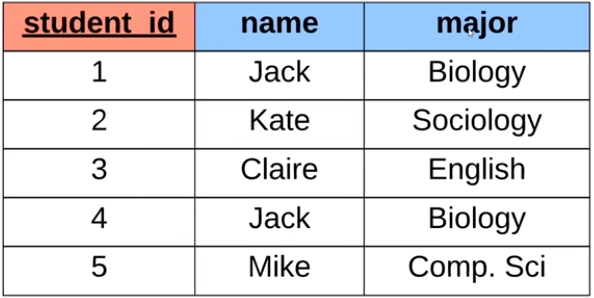
\includegraphics[width=0.4\textwidth]{./figs/example.png}
        % 	\caption{\href{}{source}}
        \end{figure}
    
    \item Use the following code:
        \begin{minted}[autogobble]{sql}
            USE giraffe;
            CREATE TABLE student (
                student_id INT,
                name VARCHAR(20),
                major VARCHAR(20),
                PRIMARY KEY(student_id)
            );

            DESCRIBE TABLE student;

            -- eliminate the table.
            DROP TABLE student;

            -- add another column called gpa.
            ALTER TABLE student ADD gpa DECIMAL;

            -- eliminate the column gpa.
            ALTER TABLE student DROP COLUMN gpa;
        \end{minted}
\end{itemize}

\section{Insert data into the database}
\begin{itemize}
    \item Using the same table as the previous section.
    \item In order to insert a piece of information to a database in SQL type the command:
        \begin{minted}[autogobble]{sql}
            INSERT INTO student VALUES(1,'Jack','Biology');
            INSERT INTO student VALUES(2,'Kate','Sociology');
        \end{minted}
    
    \item The syntax is:
        \begin{verbatim}
            INSERT INTO <table> VALUES(<values list in order>);
        \end{verbatim}
    
    \item Use the \mintinline{sql}{SELECT *} command to retrieve anything from the table:
        \begin{minted}[autogobble]{sql}
            SELECT * FROM student;
        \end{minted}
        \begin{figure}[H]
            \centering
            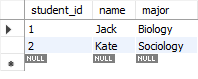
\includegraphics[width=0.4\textwidth]{./figs/insert1.png}
        % 	\caption{\href{}{source}}
        \end{figure}
    
    \item Let's say we have a student of which we do not know the major. In this case we want to modify specific attributes we must use the following syntax:
        \begin{verbatim}
            INSERT INTO student(<student_id, name>) VALUES (<new student_is, new name>);
        \end{verbatim}
        \begin{itemize}
            \item In this case since we want register a student into the database but don't know what major she is studying then we will leave that attribute as null.
        \end{itemize}
        \begin{minted}[autogobble]{sql}
            INSERT INTO student(student_id, name) VALUES (3, 'Claire');
        \end{minted}
        \begin{figure}[H]
            \centering
            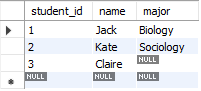
\includegraphics[width=0.4\textwidth]{./figs/insert2.png}
        % 	\caption{\href{}{source}}
        \end{figure}
    
    \item SQL will not allow you to enter duplicate keys if the key entered is a primary key, remember the primary key needs to be unique to each object.
\end{itemize}

%----------------------------------------------------------------------------------------
